%%%%%%%%%%%%%%%%%%%%%%%%%%%%%%%%%%%%%%%%%
% Structured General Purpose Assignment
% LaTeX Template
%
% This template has been downloaded from:
% http://www.latextemplates.com
%
% Original author:
% Ted Pavlic (http://www.tedpavlic.com)
%
% Note:
% The \lipsum[#] commands throughout this template generate dummy text
% to fill the template out. These commands should all be removed when 
% writing assignment content.
%
%%%%%%%%%%%%%%%%%%%%%%%%%%%%%%%%%%%%%%%%%

\documentclass{article}

\usepackage{fancyhdr} % Required for custom headers
\usepackage{lastpage} % Required to determine the last page for the footer
\usepackage{extramarks} % Required for headers and footers
\usepackage{graphicx} % Required to insert images
\usepackage[latin1]{inputenc}

% Margins
\topmargin=-0.45in
\evensidemargin=0in
\oddsidemargin=0in
\textwidth=6.5in
\textheight=9.0in
\headsep=0.25in 

\linespread{1.1} % Line spacing



\setlength\parindent{0pt} % Removes all indentation from paragraphs

%----------------------------------------------------------------------------------------
%	DOCUMENT STRUCTURE COMMANDS
%	Skip this unless you know what you're doing
%----------------------------------------------------------------------------------------

% Header and footer for when a page split occurs within a problem environment
\newcommand{\enterProblemHeader}[1]{
\nobreak\extramarks{#1}{#1 continued on next page\ldots}\nobreak
\nobreak\extramarks{#1 (continued)}{#1 continued on next page\ldots}\nobreak
}

% Header and footer for when a page split occurs between problem environments
\newcommand{\exitProblemHeader}[1]{
\nobreak\extramarks{#1 (continued)}{#1 continued on next page\ldots}\nobreak
\nobreak\extramarks{#1}{}\nobreak
}

\setcounter{secnumdepth}{0} % Removes default section numbers
\newcounter{homeworkProblemCounter} % Creates a counter to keep track of the number of problems
%----------------------------------------------------------------------------------------
%	NAME AND CLASS SECTION
%----------------------------------------------------------------------------------------

\newcommand{\lessonNumber}[1]{Lezione\ \##1} % Assignment title
\newcommand{\lessonDate}[4]{#1,\ #2\ #3\ #4} % Due date
\newcommand{\lessonCourse}[1]{#1} % Course/class
\newcommand{\lessonTime}[1]{#1} % Class/lecture time
\newcommand{\lessonTeacher}[1]{#1} % Teacher/lecturer
\newcommand{\lessonAuthor}[1]{#1} % Your name


\begin{document}

\section{Lezione 1}

% Martedì 1 Ottobre 2013

Il software, se utile, ha vita lunga.
Il ruolo di un informatico è ``al contorno della programmazione'', in modo da non produrre codice usa e getta; deve \textbf{mantenere} il software e il codice. Tutte le attività hanno un costo e non possono essere buttate al vento.

\textbf{Engineering}: ingegnere e scienziato; l'ingegnere è colui che dai principi scientifici ne trae una finalità concreta e pratica. La scienza deve scoprire questi principi e prepararli. L'ingegnere, sapendo che la scienza esiste, la applica creando qualcosa che sia \textit{mantenibile nel tempo}. Un classico esempio di engineering sono le piramidi, gli acquedotti, i ponti....

\textbf{Software}: è un terreno molto giovane, nato nella seconda guerra mondiale (40 – 45). L'ingegneria del software molto dopo. Quest'ultima non è un ramo di \textit{computer science} (ramo della scienza che spiega perché i computer sono utili) ma è una \textbf{disciplina ingegneristica} che mette insieme elementi e conoscenze. In assenza di principi ingegneristici si \textit{``fanno dei pasticci''}. Molte conoscenze vengono da campi che non sono l'informatica:

\begin{itemize}

	\item \textbf{Informatica},si vuole che un buon ingegnere del software conosca \textbf{tutte} le competenze informatiche;
	\item \textbf{Matematica}, scienza di base che aiuta a risolvere problemi;
	\item \textbf{Scienze gestionali ed economia}, è un attività di gruppo, correlazionale; è necessario capire come gestire le risorse, il tempo e il denaro;
	\item \textbf{Ingegneria}, è un pezzo di un sistema complesso che passa informazioni.
	\item \textbf{Psicologia}, il software è rilasciato con interfacce molto orientate alle persone, bisogna intercettare le aspettative di chi usa il software.

\end{itemize}

\textbf{Ciclo di vita di un software}: per regola il software nasce e ha una vita che termina con il \textbf{ritiro}. Dal momento in cui nasce esso passa in diversi \textbf{stati}, che lo fanno transire. Il software spende la maggior parte del suo tempo in uno stato che si chiama \textit{manutenzione}, in cui si possono correggere degli errori e cambiare il suo stato. Noi vorremmo una manutenzione che sia il meno invasiva possibile.

\textbf{Efficienza}: quante risorse ho impiegato per fare ciò che ho richiesto; misura il consumo e cresce al diminuire del consumo. La massima efficienza è il consumo zero (starsene seduti sul divano per intenderci), quindi da sola non basta. Le risorse che si consumano sono persone, tempo, denaro, materiale.

\textbf{Efficacia}, è una misura della conformità sul raggiungimento dell'obiettivo atteso. Si è efficaci se si raggiunge con rapidità l'obiettivo; non misura le risorse.

Bisogna cercare l'ottimo tra efficienza ed efficacia, trovare il massimo equilibrio, massimizzare gli obiettivi che sono tra l'efficienza e l'efficacia. Questi due termini sono in contrasto tra loro.

\textbf{Progetto}, \textit{assignment} (incarico): sono progetti quelli afffrontati finora, ad esempio il progetto di Programmazione ad Oggetti o il progetto di Basi di dati o Tecnologie Web. Ma tutto ciò non ha minimamente a che vedere con l'ingegneria del software: qui si parla di un incarico contrattualizzato fra parti e non più negoziabile, mentre tutto il resto è negoziabile. Verrà enfatizzato molto l'aspetto contrattuale. 

\textbf{Assignment + commitment} (impegno inderogabile): i lavori vengono dati da un assignement e trasformati in commitment.

\textbf{Engagement}: essere impegnati formalmente, impegno dal quale non si può fallire. A volte i progetti falliscono clamorosamente, per un sacco di motivi che l'ingegneria del software dovrebbe cercare alla radice. Il progetto potrebbe essere obsoleto dalla nascita, incapacità di chi ha firmato l'impegno, oppure esaurimento di tempo e/o finanziamenti. 

In questo caso vogliamo imparare come si fa a \textit{non fallire}, a soddisfare gli obiettivi entro tempi e costi noti a priori. Quante ore produttive mi servono e in quante \textit{ore di calendario} posso soddisfare determinati obiettivi (a prescindere dalle persone). Per fare ciò devo applicare principi ingegneristici. Per imbarcarsi in un progetto devo sapere che \textit{ce la posso fare}.

\textbf{Best practice}: il miglior modo di fare le cose, la selezione di ciò che è meglio fare in una certa professione.

Il termine SWE nasce nel 1968, 26 anni dopo la nascita del primo software. Dopo 45 anni la situazione è ancora terribile, la differenza è che i costi sono minori ma i prodotti buoni sono pochi.

\textbf{Stakeholder}: è una persona che conta, un portatore di interesse, che ha influenza sul prodotto.

\fbox{L'approccio \textbf{sistematico}, \textbf{disciplinato} e \textbf{quantificabile} allo sviluppo, uso, manutenzione e ritiro del software}

\textbf{Sistematico}: agisco secondo un sistema, affronto il medesimo problema sempre nello stesso modo (nel modo giusto), senza improvvisazione o creatività.

\textbf{Disciplinato}: ciascuno fa il suo e nessuno fallisce, perchè l'ingegneria del software è un'attività collaborativa. Seguire in modo rigoroso la disciplina è nostro dovere, produce affidabilità.

\textbf{Quantificabile}: esprimere una quantità; se sono sistematico e disciplinato saprò dire a priori quanto tempo mi ci vorrà per fare una cosa. Si può essere quantificabili solo se si è sistematici e disciplinati. Noi cerchiamo un approccio con queste caratteristiche.

\begin{center}

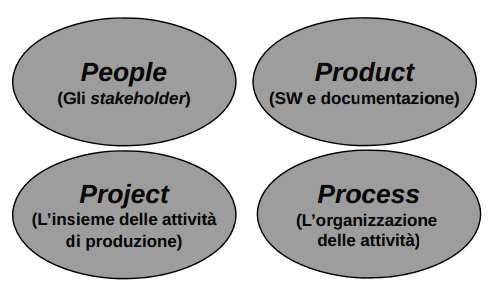
\includegraphics[width=0.75\columnwidth]{img1} % Example image

\end{center}

\begin{itemize}

	\item \textbf{People}: insieme delle persone che commissionano e ricevono;

	\item \textbf{Product}: il sw è parte di un sistema complesso;

	\item \textbf{Process}: l'insieme di attività che svolgiamo ad un particolare fine;

	\item \textbf{Project}: attività specifiche svolte a fronte di un assignment che diventa un commitment.

\end{itemize}

Tre strati:

\begin{itemize}

	\item \textbf{Customer}: il cliente, quello che ha un bisogno espresso o inespresso; due poli, gli stakeholder che costruiscono le \textit{opportunità};
	\item \textbf{Solution}: dove esiste il customer c'è qualcuno che trova una soluzione, fatta di \textbf{requisiti} (di cosa c'è bisogno);
	\item \textbf{Endeavor}: l'impegno per realizzare il software, il team interagisce con gli stakeholder; l'ingegneria del software è un'attività strettamente collaborativa, ho bisogno di un metodo di lavoro per il team, di una \textit{Way of working}.

\end{itemize}

\textbf{SWE != PROGRAMMING}: la programmazione è solo un elemento, e anche il meno importante. Il programmatore deve fare solo quello che viene chiesto (da un membro del team stesso). Il programmatore deve obbedire, non può essere creativo.

Principi etici:

\begin{itemize}

	\item Considerare la qualità come primo obiettivo;
	\item Produrre sw di qualità è possibile;
	\item Aiutare il cliente a comprendere i suoi veri bisogni;
	\item Adottare i processi più adatti al progetto;
	\item Ridurre la distanza intellettuale tra il sw e il problema da risolvere;
	\item Essere proattivi nel cercare e rimuovere gli errori;
	\item Motivare, formare, far crescere le persone.

\end{itemize}

\end{document}